\documentclass{standalone}

\usepackage{microtype}
\usepackage[utf8]{inputenc}
\usepackage[mono=false]{libertine}

\usepackage{pgfplots}
\usepgfplotslibrary{external}

\usepackage{tikz}
\usetikzlibrary{shapes.geometric, arrows, calc}

\tikzstyle{outcome} = [rectangle, draw=black]
\tikzstyle{child} = [rectangle, rounded corners, fill=green!30, draw=black]
\tikzstyle{p1} = [rectangle, rounded corners, fill=red!30, draw=black]
\tikzstyle{p2} = [rectangle, rounded corners, fill=blue!30, draw=black]

\tikzstyle{arrow} = [thick,->]
\tikzstyle{dblarr} = [<->]

\newcommand{\vrrsbcov}{$38.0$}
\newcommand{\bapqcov}{$0.05$}
\newcommand{\gendercov}{$-0.2$}
\newcommand{\educcov}{$0.25$}
\newcommand{\tswccov}{$26.4$}

\newcommand{\agepcg}{$-2.0$}
\newcommand{\agescg}{$-0.4$}
\newcommand{\sexpcg}{$3.4$}
\newcommand{\sexscg}{$2.4$}

\newcommand{\bapqpcg}{$6.0$}
\newcommand{\bapqscg}{$3.7$}

% format: pcg/scg outcome~cov

\newcommand{\pcgedgender}{$-1.0$}
\newcommand{\pcgedbapq}{$-1.3$}
\newcommand{\pcgtswcgender}{$-5.3$}
\newcommand{\pcgtswced}{$-0.7$}

\newcommand{\scgedgender}{$-1.1$}
\newcommand{\scgedbapq}{$-3.9$}
\newcommand{\scgtswcgender}{$-1.3$}
\newcommand{\scgtswced}{$-0.07$}

\newcommand{\ns}[1]{\textit{#1\textsuperscript{n.s.}}}

%\tikzexternalize[prefix={tikz_external/}, only named]
%\tikzsetnextfilename{vrs}

\newcommand{\total}{vrRSB\textsubscript{T}}

\begin{document}

    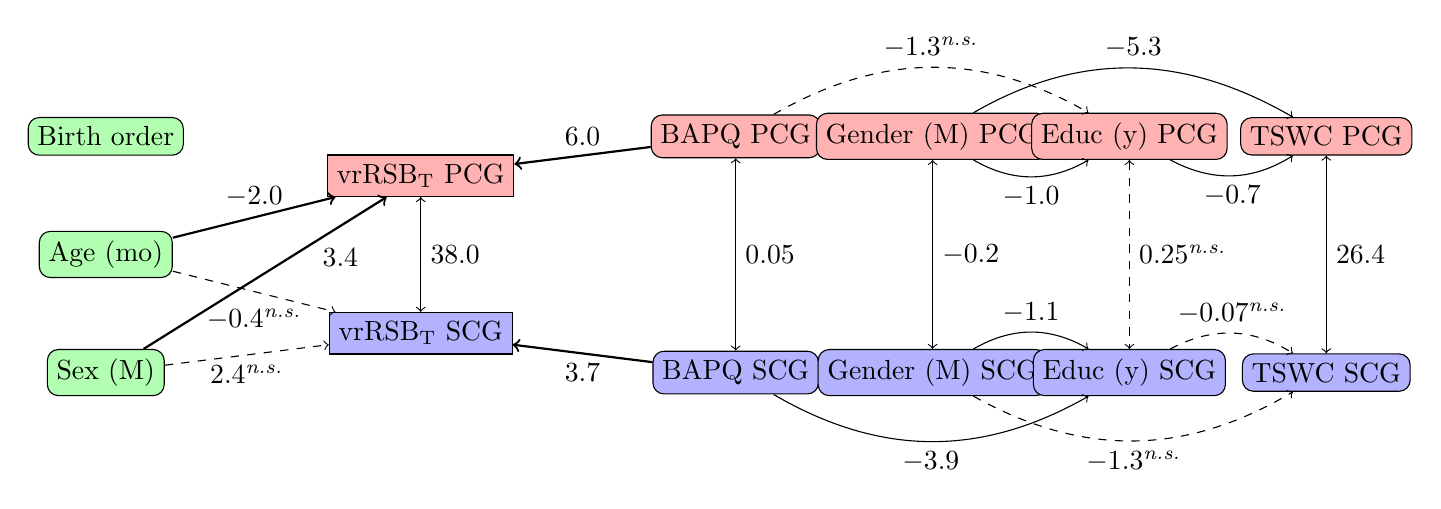
\begin{tikzpicture}

        \node (vrs1) [outcome, fill=red!30] {\total{} PCG};
        \node (vrs2) [outcome, fill=blue!30, below of=vrs1,
                        node distance=2cm] {\total{} SCG};
        \node (vrscenter) at ($(vrs1)!0.5!(vrs2)$) {} ;

        % Place this stack of nodes to the left of the center of the things
        \node (age) [child, left of=vrscenter,
                        node distance=4cm] {Age (mo)} ;
        \node (bo)  [child, above of=age, node distance=1.5cm] {Birth order} ;
        \node (sex) [child, below of=age, node distance=1.5cm] {Sex (M)} ;

        % arrows
        \draw [dblarr] (vrs1) -- node[anchor=west] {\vrrsbcov} (vrs2) ;

        %age
        \draw [arrow] (age) -- node[anchor=south] {\agepcg} (vrs1) ;
        \draw [->,dashed]
            (age)  --
                node[anchor=north,yshift=-0.1cm] {\ns{\agescg}}
            (vrs2) ;

        \draw [arrow]
            (sex) --
                node[anchor=west,xshift=0.6cm,yshift=0.2cm] {\sexpcg}
            (vrs1) ;

        \draw [->,dashed] (sex) -- node[anchor=north] {\ns{\sexscg}} (vrs2) ;

        % PARENTS ====

        \node (parentcenter) [right of=vrscenter, node distance=4cm] {} ;

        \node (p1bapq) [p1, above of=parentcenter, node distance=1.5cm]
            {BAPQ  PCG} ;
        \node (p1gender) [p1, right of=p1bapq, node distance=2.5cm]
            {Gender (M) PCG} ;
        \node (p1educ) [p1, right of=p1gender, node distance=2.5cm]
            {Educ (y) PCG} ;
        \node (p1tswc) [p1, right of=p1educ, node distance=2.5cm] {TSWC PCG} ;

        \node (p2bapq) [p2, below of=parentcenter, node distance=1.5cm]
            {BAPQ SCG} ;
        \node (p2gender) [p2, right of=p2bapq, node distance=2.5cm]
            {Gender (M) SCG} ;
        \node (p2educ) [p2, right of=p2gender, node distance=2.5cm]
            {Educ (y) SCG} ;
        \node (p2tswc) [p2, right of=p2educ, node distance=2.5cm] {TSWC SCG} ;

        \draw [dblarr] (p1bapq) --   node[anchor=west] {\bapqcov} (p2bapq) ;
        \draw [dblarr] (p1gender) -- node[anchor=west] {\gendercov} (p2gender) ;
        \draw [dblarr,dashed]
            (p1educ) --
                node[anchor=west] {\ns{\educcov}}
            (p2educ) ;
        \draw [dblarr] (p1tswc) --   node[anchor=west] {\tswccov} (p2tswc) ;

        % PCG

        \draw [->]
            (p1gender) to
                [bend right]
                node[anchor=north]{\pcgedgender}
            (p1educ) ;

        \draw [->,dashed]
            (p1bapq) to
                [out=30,in=150]
                node[anchor=south] {\ns{\pcgedbapq}}
            (p1educ) ;

        \draw [->]
            (p1educ) to
                [bend right]
                node[anchor=north] {\pcgtswced}
            (p1tswc) ;

        \draw [->]
            (p1gender) to
                [out=30,in=150]
                node[anchor=south] {\pcgtswcgender}
            (p1tswc) ;

%        \draw [<->,dotted] (p2educ) to
%            [out=30,in=150]
%            (p2bapq) ;

        % SCG

%        \draw [->] (p2gender) to [out=150, in=30] (p2bapq) ;
        \draw [->]
            (p2gender) to
                [bend left, out=30,in=150]
                node[anchor=south] {\scgedgender}
            (p2educ) ;

        \draw [->]
            (p2bapq) to
                [bend right]
                node[anchor=north] {\scgedbapq}
            (p2educ) ;

        \draw [->,dashed]
            (p2educ) to
                [bend left]
                node[anchor=south] {\ns{\scgtswced}}
            (p2tswc) ;

        \draw [->,dashed]
            (p2gender) to
                [bend right]
                node[anchor=north] {\ns{\scgtswcgender}}
            (p2tswc) ;

        % bapq effects
        \draw [arrow,thick] (p1bapq) -- node[anchor=south] {\bapqpcg} (vrs1) ;

        \draw [arrow,thick] (p2bapq) -- node[anchor=north] {\bapqscg} (vrs2) ;

    \end{tikzpicture}


\end{document}